% Options for packages loaded elsewhere
% Options for packages loaded elsewhere
\PassOptionsToPackage{unicode}{hyperref}
\PassOptionsToPackage{hyphens}{url}
\PassOptionsToPackage{dvipsnames,svgnames,x11names}{xcolor}
%
\documentclass[
  12pt]{article}
\usepackage{xcolor}
\usepackage{amsmath,amssymb}
\setcounter{secnumdepth}{5}
\usepackage{iftex}
\ifPDFTeX
  \usepackage[T1]{fontenc}
  \usepackage[utf8]{inputenc}
  \usepackage{textcomp} % provide euro and other symbols
\else % if luatex or xetex
  \usepackage{unicode-math} % this also loads fontspec
  \defaultfontfeatures{Scale=MatchLowercase}
  \defaultfontfeatures[\rmfamily]{Ligatures=TeX,Scale=1}
\fi
\usepackage{lmodern}
\ifPDFTeX\else
  % xetex/luatex font selection
\fi
% Use upquote if available, for straight quotes in verbatim environments
\IfFileExists{upquote.sty}{\usepackage{upquote}}{}
\IfFileExists{microtype.sty}{% use microtype if available
  \usepackage[]{microtype}
  \UseMicrotypeSet[protrusion]{basicmath} % disable protrusion for tt fonts
}{}
\makeatletter
\@ifundefined{KOMAClassName}{% if non-KOMA class
  \IfFileExists{parskip.sty}{%
    \usepackage{parskip}
  }{% else
    \setlength{\parindent}{0pt}
    \setlength{\parskip}{6pt plus 2pt minus 1pt}}
}{% if KOMA class
  \KOMAoptions{parskip=half}}
\makeatother
% Make \paragraph and \subparagraph free-standing
\makeatletter
\ifx\paragraph\undefined\else
  \let\oldparagraph\paragraph
  \renewcommand{\paragraph}{
    \@ifstar
      \xxxParagraphStar
      \xxxParagraphNoStar
  }
  \newcommand{\xxxParagraphStar}[1]{\oldparagraph*{#1}\mbox{}}
  \newcommand{\xxxParagraphNoStar}[1]{\oldparagraph{#1}\mbox{}}
\fi
\ifx\subparagraph\undefined\else
  \let\oldsubparagraph\subparagraph
  \renewcommand{\subparagraph}{
    \@ifstar
      \xxxSubParagraphStar
      \xxxSubParagraphNoStar
  }
  \newcommand{\xxxSubParagraphStar}[1]{\oldsubparagraph*{#1}\mbox{}}
  \newcommand{\xxxSubParagraphNoStar}[1]{\oldsubparagraph{#1}\mbox{}}
\fi
\makeatother

\usepackage{color}
\usepackage{fancyvrb}
\newcommand{\VerbBar}{|}
\newcommand{\VERB}{\Verb[commandchars=\\\{\}]}
\DefineVerbatimEnvironment{Highlighting}{Verbatim}{commandchars=\\\{\}}
% Add ',fontsize=\small' for more characters per line
\usepackage{framed}
\definecolor{shadecolor}{RGB}{241,243,245}
\newenvironment{Shaded}{\begin{snugshade}}{\end{snugshade}}
\newcommand{\AlertTok}[1]{\textcolor[rgb]{0.68,0.00,0.00}{#1}}
\newcommand{\AnnotationTok}[1]{\textcolor[rgb]{0.37,0.37,0.37}{#1}}
\newcommand{\AttributeTok}[1]{\textcolor[rgb]{0.40,0.45,0.13}{#1}}
\newcommand{\BaseNTok}[1]{\textcolor[rgb]{0.68,0.00,0.00}{#1}}
\newcommand{\BuiltInTok}[1]{\textcolor[rgb]{0.00,0.23,0.31}{#1}}
\newcommand{\CharTok}[1]{\textcolor[rgb]{0.13,0.47,0.30}{#1}}
\newcommand{\CommentTok}[1]{\textcolor[rgb]{0.37,0.37,0.37}{#1}}
\newcommand{\CommentVarTok}[1]{\textcolor[rgb]{0.37,0.37,0.37}{\textit{#1}}}
\newcommand{\ConstantTok}[1]{\textcolor[rgb]{0.56,0.35,0.01}{#1}}
\newcommand{\ControlFlowTok}[1]{\textcolor[rgb]{0.00,0.23,0.31}{\textbf{#1}}}
\newcommand{\DataTypeTok}[1]{\textcolor[rgb]{0.68,0.00,0.00}{#1}}
\newcommand{\DecValTok}[1]{\textcolor[rgb]{0.68,0.00,0.00}{#1}}
\newcommand{\DocumentationTok}[1]{\textcolor[rgb]{0.37,0.37,0.37}{\textit{#1}}}
\newcommand{\ErrorTok}[1]{\textcolor[rgb]{0.68,0.00,0.00}{#1}}
\newcommand{\ExtensionTok}[1]{\textcolor[rgb]{0.00,0.23,0.31}{#1}}
\newcommand{\FloatTok}[1]{\textcolor[rgb]{0.68,0.00,0.00}{#1}}
\newcommand{\FunctionTok}[1]{\textcolor[rgb]{0.28,0.35,0.67}{#1}}
\newcommand{\ImportTok}[1]{\textcolor[rgb]{0.00,0.46,0.62}{#1}}
\newcommand{\InformationTok}[1]{\textcolor[rgb]{0.37,0.37,0.37}{#1}}
\newcommand{\KeywordTok}[1]{\textcolor[rgb]{0.00,0.23,0.31}{\textbf{#1}}}
\newcommand{\NormalTok}[1]{\textcolor[rgb]{0.00,0.23,0.31}{#1}}
\newcommand{\OperatorTok}[1]{\textcolor[rgb]{0.37,0.37,0.37}{#1}}
\newcommand{\OtherTok}[1]{\textcolor[rgb]{0.00,0.23,0.31}{#1}}
\newcommand{\PreprocessorTok}[1]{\textcolor[rgb]{0.68,0.00,0.00}{#1}}
\newcommand{\RegionMarkerTok}[1]{\textcolor[rgb]{0.00,0.23,0.31}{#1}}
\newcommand{\SpecialCharTok}[1]{\textcolor[rgb]{0.37,0.37,0.37}{#1}}
\newcommand{\SpecialStringTok}[1]{\textcolor[rgb]{0.13,0.47,0.30}{#1}}
\newcommand{\StringTok}[1]{\textcolor[rgb]{0.13,0.47,0.30}{#1}}
\newcommand{\VariableTok}[1]{\textcolor[rgb]{0.07,0.07,0.07}{#1}}
\newcommand{\VerbatimStringTok}[1]{\textcolor[rgb]{0.13,0.47,0.30}{#1}}
\newcommand{\WarningTok}[1]{\textcolor[rgb]{0.37,0.37,0.37}{\textit{#1}}}

\usepackage{longtable,booktabs,array}
\usepackage{calc} % for calculating minipage widths
% Correct order of tables after \paragraph or \subparagraph
\usepackage{etoolbox}
\makeatletter
\patchcmd\longtable{\par}{\if@noskipsec\mbox{}\fi\par}{}{}
\makeatother
% Allow footnotes in longtable head/foot
\IfFileExists{footnotehyper.sty}{\usepackage{footnotehyper}}{\usepackage{footnote}}
\makesavenoteenv{longtable}
\usepackage{graphicx}
\makeatletter
\newsavebox\pandoc@box
\newcommand*\pandocbounded[1]{% scales image to fit in text height/width
  \sbox\pandoc@box{#1}%
  \Gscale@div\@tempa{\textheight}{\dimexpr\ht\pandoc@box+\dp\pandoc@box\relax}%
  \Gscale@div\@tempb{\linewidth}{\wd\pandoc@box}%
  \ifdim\@tempb\p@<\@tempa\p@\let\@tempa\@tempb\fi% select the smaller of both
  \ifdim\@tempa\p@<\p@\scalebox{\@tempa}{\usebox\pandoc@box}%
  \else\usebox{\pandoc@box}%
  \fi%
}
% Set default figure placement to htbp
\def\fps@figure{htbp}
\makeatother





\setlength{\emergencystretch}{3em} % prevent overfull lines

\providecommand{\tightlist}{%
  \setlength{\itemsep}{0pt}\setlength{\parskip}{0pt}}



 
\usepackage[]{natbib}
\bibliographystyle{agsm}


\addtolength{\oddsidemargin}{-.5in}%
\addtolength{\evensidemargin}{-1in}%
\addtolength{\textwidth}{1in}%
\addtolength{\textheight}{1.7in}%
\addtolength{\topmargin}{-1in}%
\usepackage{booktabs}
\usepackage{longtable}
\usepackage{array}
\usepackage{multirow}
\usepackage{wrapfig}
\usepackage{float}
\usepackage{colortbl}
\usepackage{pdflscape}
\usepackage{tabu}
\usepackage{threeparttable}
\usepackage{threeparttablex}
\usepackage[normalem]{ulem}
\usepackage{makecell}
\usepackage{xcolor}
\makeatletter
\@ifpackageloaded{caption}{}{\usepackage{caption}}
\AtBeginDocument{%
\ifdefined\contentsname
  \renewcommand*\contentsname{Table of contents}
\else
  \newcommand\contentsname{Table of contents}
\fi
\ifdefined\listfigurename
  \renewcommand*\listfigurename{List of Figures}
\else
  \newcommand\listfigurename{List of Figures}
\fi
\ifdefined\listtablename
  \renewcommand*\listtablename{List of Tables}
\else
  \newcommand\listtablename{List of Tables}
\fi
\ifdefined\figurename
  \renewcommand*\figurename{Figure}
\else
  \newcommand\figurename{Figure}
\fi
\ifdefined\tablename
  \renewcommand*\tablename{Table}
\else
  \newcommand\tablename{Table}
\fi
}
\@ifpackageloaded{float}{}{\usepackage{float}}
\floatstyle{ruled}
\@ifundefined{c@chapter}{\newfloat{codelisting}{h}{lop}}{\newfloat{codelisting}{h}{lop}[chapter]}
\floatname{codelisting}{Listing}
\newcommand*\listoflistings{\listof{codelisting}{List of Listings}}
\makeatother
\makeatletter
\makeatother
\makeatletter
\@ifpackageloaded{caption}{}{\usepackage{caption}}
\@ifpackageloaded{subcaption}{}{\usepackage{subcaption}}
\makeatother
\usepackage{bookmark}
\IfFileExists{xurl.sty}{\usepackage{xurl}}{} % add URL line breaks if available
\urlstyle{same}
\hypersetup{
  pdftitle={Final Project Title},
  pdfauthor={YourName},
  pdfkeywords={3 to 6 keywords, that do not appear in the title},
  colorlinks=true,
  linkcolor={blue},
  filecolor={Maroon},
  citecolor={Blue},
  urlcolor={Blue},
  pdfcreator={LaTeX via pandoc}}



\begin{document}


\def\spacingset#1{\renewcommand{\baselinestretch}%
{#1}\small\normalsize} \spacingset{1}


%%%%%%%%%%%%%%%%%%%%%%%%%%%%%%%%%%%%%%%%%%%%%%%%%%%%%%%%%%%%%%%%%%%%%%%%%%%%%%

\date{November 4, 2025}
\title{\bf Final Project Title}
\author{
YourName\thanks{The author gratefully acknowledges \emph{put your thanks
here - can wait till final version to input anything, thank friends,
peer who did your peer review, parents/guardians, whoever you'd like to
acknowledge}.}\\
Department of Statistics, Amherst College\\
}
\maketitle

\bigskip
\bigskip
\begin{abstract}
The text of your abstract. 200 or fewer words. It is intended to provide
an overview of your paper and may be similar to your synopsis. Note that
an abstract can only include one paragraph in this format. You may want
to put your synopsis here as you work to refer to it easily.
\end{abstract}

\noindent%
{\it Keywords:} 3 to 6 keywords, that do not appear in the title
\vfill

\newpage
\spacingset{1.9} % DON'T change the spacing!


\section{Introduction}\label{sec-intro}

Body of paper. Margins in this document are roughly 0.75 inches all
around, letter size paper.

This template will be used for you to submit your final project. You
need to copy over the PaperTemplate folder in its entirety. Make sure
you have the agsm.bst file and bibliography.bib file in order to render
to pdf. If you make your own bibliography.bib file later, that's fine -
change the name above to match your file name, though for a lot of folks
you'll just edit the bibliography.bib file provided. If you don't use a
reference in it, it won't print, so you can keep the examples below and
drop them at the end and they will disappear (or drop them once you have
your own examples in to reference). You'll want the setup for the file
to look the same in your repo as in the class repo. You should change
the name of the file to something other than ``template'' at some point
though - ``draft'' or ``finalreport'', etc when it gets closer to time.
Remember that if something goes wrong with the file, you can always look
back at the class repo for the original files and their structure, or
grab a new copy of the ``template'' file.

\section{Methods}\label{sec-meth}

Don't take any of these section titles seriously. They're just for
illustration.

\section{Verifications}\label{sec-verify}

What can we do with the template? References and citations are a big
thing to figure out!

We can refer to sections (e.g., this is section \ref{sec-verify}, while
the previous section was section \ref{sec-meth}). Sub-section references
are demo-ed below.

We cite using the BibTeX system. Here we can reference papers by
\citet{Campbell02} and \citet{Schubert13} through inline citations (see
the \texttt{bibliography.bib} file for the reference database).

More work that is relevant can also be cited in a traditional fashion
\citep[\citet{Galyardt14mmm}, \citet{Galyardt12dis}]{Chi81}.

Note that you can capitalize proper nouns in citations
\citep{Campbell02} (again, see \texttt{bibliography.bib}).

We also test some other ways to do the citations, such as \cite{Chi81},
and \citep{Campbell02}. These both work. The latter puts the citation in
parentheses. You can also use \citet{Chi81}, though this seems to have
similar behavior to just cite.

The original citation examples in the template were:

\citet{gelm:veht:2021} offer some guidance about key ideas about
statistical ideas. On an unrelated note, spreadsheets are important to
use correctly \citep{brom:woo:2018}. Log-linear models are an attractive
way to model categorical data \citep{bish:fien:1975}.

Note the different structure used in the examples if it is at the end of
a sentence/paragraph versus if you are using it as part of the sentence.

Your exposition section (where you have new material) should likely have
one citation per paragraph at a minimum where you are pulling from new
sources. The idea is to cite where you got your material. Let's look at
an example paragraph structure.

This is my intro sentence. I took this idea from source 1. This sentence
also paraphrases an idea from source 1 \citep{Campbell02}. Now I am
moving onto something else and it's my own example, so I don't need to
cite. Still my own example/words. However, I want to close with
something from a different source \citep{Chi81}.

If the entire paragraph paraphrases from a single source, it only need a
single citation at the end. But you should cite before you go into your
own examples, etc. That may mean citing the same source in the same
paragraph in different places.

You don't need to cite every sentence, unless swapping sources.

These next sections will be just long enough to illustrate what a full
page of text looks like, for margins and spacing.

The quick brown fox jumped over the lazy dog. The quick brown fox jumped
over the lazy dog. The quick brown fox jumped over the lazy dog. The
quick brown fox jumped over the lazy dog. The quick brown fox jumped
over the lazy dog. The quick brown fox jumped over the lazy dog. The
quick brown fox jumped over the lazy dog. The quick brown fox jumped
over the lazy dog. The quick brown fox jumped over the lazy dog.

The quick brown fox jumped over the lazy dog. The quick brown fox jumped
over the lazy dog. The quick brown fox jumped over the lazy dog. The
quick brown fox jumped over the lazy dog. The quick brown fox jumped
over the lazy dog. The quick brown fox jumped over the lazy dog. The
quick brown fox jumped over the lazy dog. The quick brown fox jumped
over the lazy dog. The quick brown fox jumped over the lazy dog. The
quick brown fox jumped over the lazy dog.

\subsection{Example Subsection}\label{sec-verify-sub1}

You can reference subsections too. This is subsection
\ref{sec-verify-sub1}.

The quick brown fox jumped over the lazy dog. The quick brown fox jumped
over the lazy dog. The quick brown fox jumped over the lazy dog. The
quick brown fox jumped over the lazy dog. The quick brown fox jumped
over the lazy dog. The quick brown fox jumped over the lazy dog. The
quick brown fox jumped over the lazy dog. The quick brown fox jumped
over the lazy dog. The quick brown fox jumped over the lazy dog. The
quick brown fox jumped over the lazy dog.

The quick brown fox jumped over the lazy dog. The quick brown fox jumped
over the lazy dog. The quick brown fox jumped over the lazy dog. The
quick brown fox jumped over the lazy dog. The quick brown fox jumped
over the lazy dog. The quick brown fox jumped over the lazy dog. The
quick brown fox jumped over the lazy dog. The quick brown fox jumped
over the lazy dog. The quick brown fox jumped over the lazy dog. The
quick brown fox jumped over the lazy dog.

The quick brown fox jumped over the lazy dog. The quick brown fox jumped
over the lazy dog. The quick brown fox jumped over the lazy dog.

\subsection{Another Example
Subsection}\label{another-example-subsection}

The quick brown fox jumped over the lazy dog. The quick brown fox jumped
over the lazy dog. The quick brown fox jumped over the lazy dog. The
quick brown fox jumped over the lazy dog. The quick brown fox jumped
over the lazy dog. The quick brown fox jumped over the lazy dog. The
quick brown fox jumped over the lazy dog. The quick brown fox jumped
over the lazy dog. The quick brown fox jumped over the lazy dog. The
quick brown fox jumped over the lazy dog.

The quick brown fox jumped over the lazy dog. The quick brown fox jumped
over the lazy dog. The quick brown fox jumped over the lazy dog. The
quick brown fox jumped over the lazy dog. The quick brown fox jumped
over the lazy dog. The quick brown fox jumped over the lazy dog. The
quick brown fox jumped over the lazy dog. The quick brown fox jumped
over the lazy dog. The quick brown fox jumped over the lazy dog. The
quick brown fox jumped over the lazy dog.

The quick brown fox jumped over the lazy dog. The quick brown fox jumped
over the lazy dog. The quick brown fox jumped over the lazy dog. The
quick brown fox jumped over the lazy dog. The quick brown fox jumped
over the lazy dog. The quick brown fox jumped over the lazy dog. The
quick brown fox jumped over the lazy dog. The quick brown fox jumped
over the lazy dog. The quick brown fox jumped over the lazy dog. The
quick brown fox jumped over the lazy dog.

\section{Examples}\label{examples}

Lots of things can be done in this template. Multiple ways of including
figures and tables and referencing them are demo-ed below.

\begin{figure}

\centering{

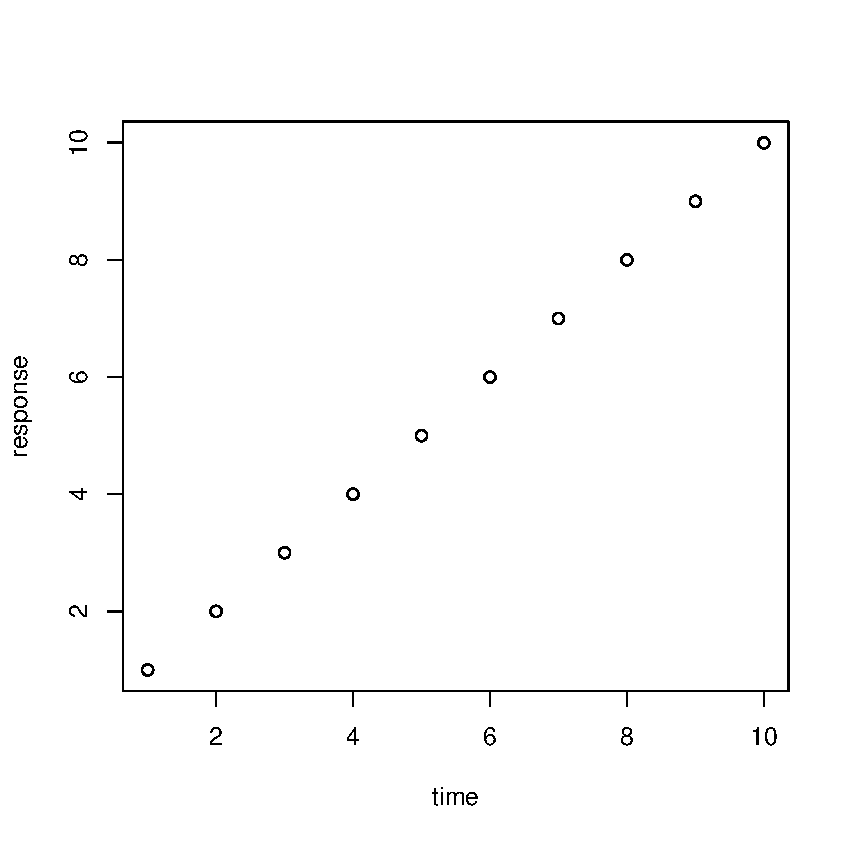
\includegraphics[width=3in,height=\textheight,keepaspectratio]{fig1.pdf}

}

\caption{\label{fig-first}Consistency comparison in fitting surrogate
model in the tidal power example.}

\end{figure}%

\begin{longtable}[]{@{}lllll@{}}
\caption{D-optimality values for design X under five different
scenarios.}\label{tbl-one}\tabularnewline
\toprule\noalign{}
one & two & three & four & five \\
\midrule\noalign{}
\endfirsthead
\toprule\noalign{}
one & two & three & four & five \\
\midrule\noalign{}
\endhead
\bottomrule\noalign{}
\endlastfoot
1.23 & 3.45 & 5.00 & 1.21 & 3.41 \\
1.23 & 3.45 & 5.00 & 1.21 & 3.42 \\
1.23 & 3.45 & 5.00 & 1.21 & 3.43 \\
\end{longtable}

You can reference these as Figure~\ref{fig-first} and
Table~\ref{tbl-one}.

What if you are generating the table via code? (Probably what you are
doing.) No problem!

\begin{Shaded}
\begin{Highlighting}[]
\NormalTok{iris }\SpecialCharTok{\%\textgreater{}\%}
  \FunctionTok{group\_by}\NormalTok{(Species) }\SpecialCharTok{\%\textgreater{}\%}
  \FunctionTok{summarize}\NormalTok{(}\AttributeTok{count =} \FunctionTok{n}\NormalTok{()) }\SpecialCharTok{\%\textgreater{}\%}
\NormalTok{  knitr}\SpecialCharTok{::}\FunctionTok{kable}\NormalTok{()}
\end{Highlighting}
\end{Shaded}

\begin{longtable}[]{@{}lr@{}}

\caption{\label{tbl-demotable}This is a sample table caption that should
interpret the table!}

\tabularnewline

\toprule\noalign{}
Species & count \\
\midrule\noalign{}
\endhead
\bottomrule\noalign{}
\endlastfoot
setosa & 50 \\
versicolor & 50 \\
virginica & 50 \\

\end{longtable}

Table~\ref{tbl-demotable} displays the number of irises per species. As
long as you use the tbl and fig prefixes, it will keep track and you
don't have to!

\begin{Shaded}
\begin{Highlighting}[]
\NormalTok{iris }\SpecialCharTok{\%\textgreater{}\%} 
  \FunctionTok{ggplot}\NormalTok{(}\FunctionTok{aes}\NormalTok{(}\AttributeTok{y =}\NormalTok{ Sepal.Width, }\AttributeTok{color =}\NormalTok{ Species)) }\SpecialCharTok{+}
  \FunctionTok{geom\_boxplot}\NormalTok{()}
\end{Highlighting}
\end{Shaded}

\begin{figure}[H]

\centering{

\pandocbounded{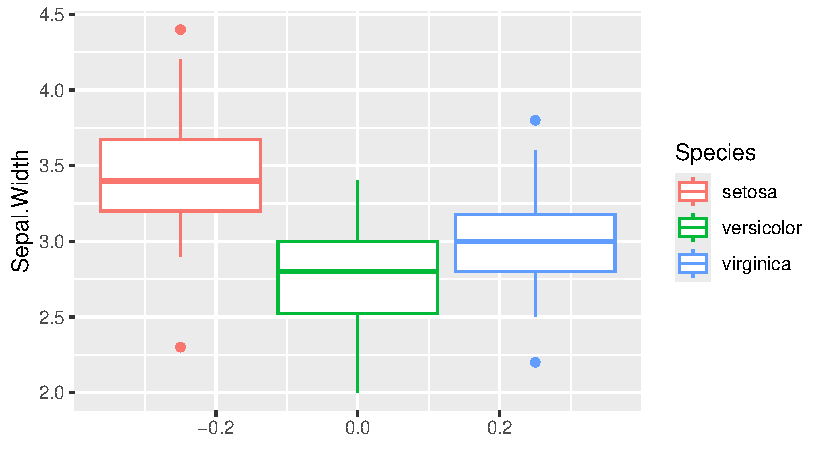
\includegraphics[keepaspectratio]{template_files/figure-pdf/fig-irisdemo-1.pdf}}

}

\caption{\label{fig-irisdemo}This is a sample figure caption that should
interpret the figure!}

\end{figure}%

Similarly, we can reference figures generated by our code.
Figure~\ref{fig-irisdemo} displays the side-by-side boxplots for
Sepal.Width by Species.

You can bring in other images if appropriate (need to cite if it's not
something you generated). Figure~\ref{fig-campusmap} displays a campus
map.

\begin{Shaded}
\begin{Highlighting}[]
\NormalTok{knitr}\SpecialCharTok{::}\FunctionTok{include\_graphics}\NormalTok{(}\StringTok{"campus\_map.png"}\NormalTok{)}
\end{Highlighting}
\end{Shaded}

\begin{figure}[H]

\centering{

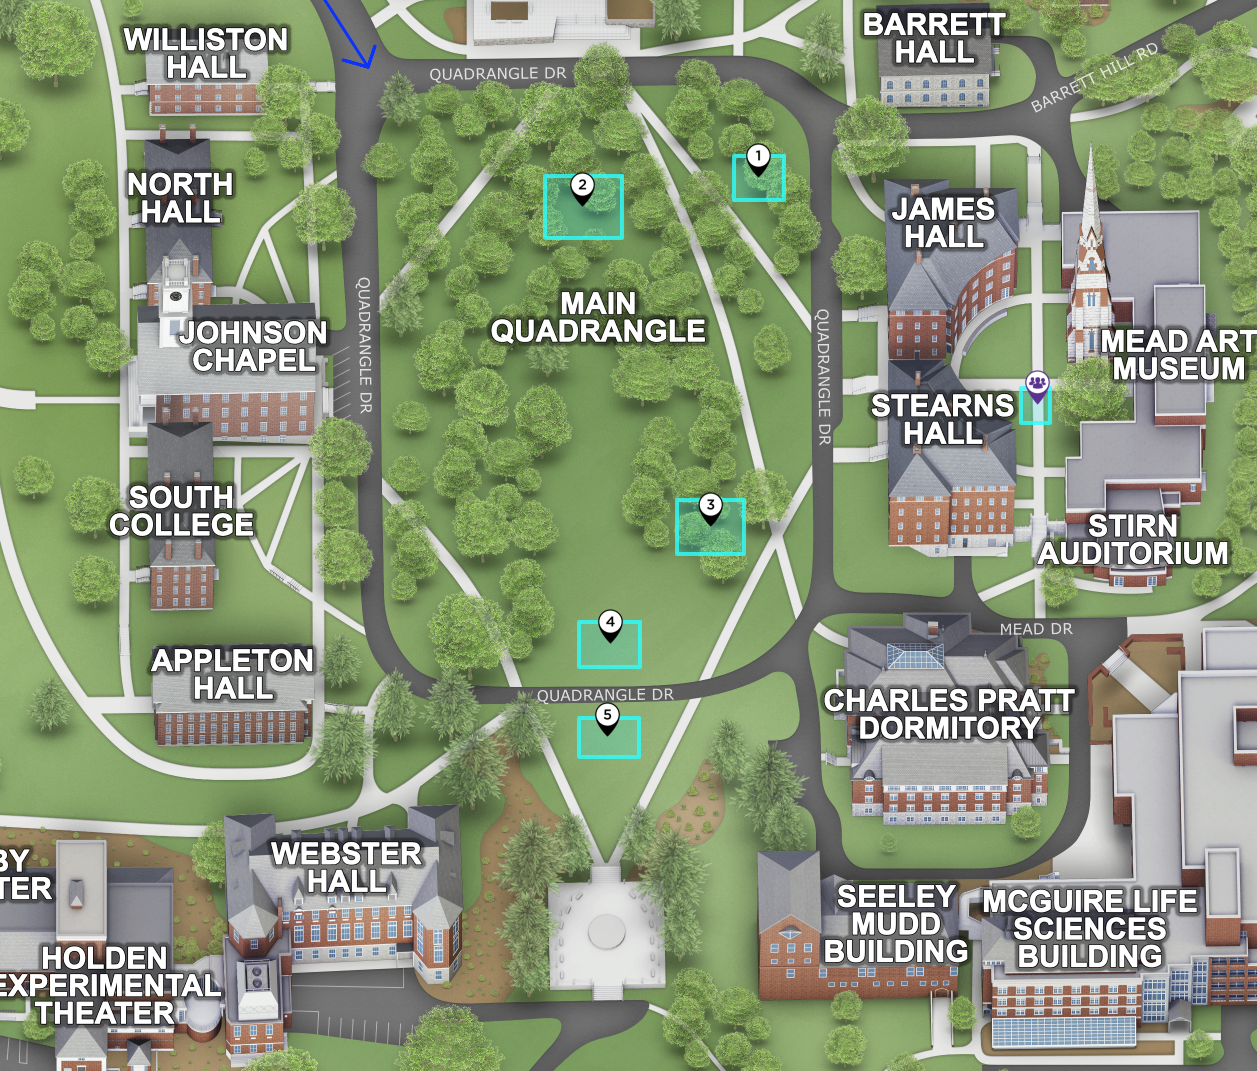
\includegraphics[width=0.8\linewidth,height=\textheight,keepaspectratio]{campus_map.png}

}

\caption{\label{fig-campusmap}Another sample figure caption}

\end{figure}%

\section{LaTeX Examples}\label{latex-examples}

To shift into ``tex'' mode while in-line, it's pretty easy. You just
need dollar signs.

The variables \(X_1\) and \(X_2\) are uncorrelated.

If you have multiple indices or items that need to go into a subscript
or a superscript, you need curly brackets.

We want to look at \(X_{10}\) and \(X_{10}^{20}\).

If you have a big equation, you probably want to set it on it's own,
rather than try it in-line. That means DOUBLE dollar signs in Qmds. It
doesn't like a different framework you might have seen in .Rmds. And
yes, it seems to ``add space'', but that's ok. Just run with it (if I
can figure out how to edit it, will let you know!).

In regression, we assert (for two predictor variables) that

\[
\mu_Y = \beta_0 + \beta_1X_1 + \beta_2X_2.
\]

Don't forget punctuation in your equations.

If you want to reference equations, you need to be a bit more formal:

\begin{equation}
\label{regeq}
\mu_Y = \beta_0 + \beta_1X_1 + \beta_2X_2.
\end{equation}

Now I can refer to the equation as Equation \ref{regeq}.

I'm going to borrow a lot of the examples below from the revision of my
Probability textbook, so if the context is a little strange (meaning,
not from our class), that's why.

You can do bulleted lists using LaTeX instead of RMarkdown formatting
like this:

\begin{enumerate}
\item ``Define the terms: continuous RV, probability density function, and cumulative density function.
\item Compute expectation and variance for continuous RVs.
\item Apply uniform and exponential distributions to appropriate problems.
\item Solve problems involving joint and marginal distributions in the continuous setting.
\item Extend independence, covariance, and correlation concepts to the continuous setting.
\item Work with uniform and exponential distributions in R to find probabilities and simulate problems.'' (Chapter 6 introduction)
\end{enumerate}

In equations, you can also do alignments and adjust spacing with various
commands. In text, you can also get italics and bold text. Here is some
text with examples of these, including fractions in the equations.

``That is, we integrate a constant \(c\) over the bullseye region. This
leads to

\begin{align}
\label{pofb}
P(B) = \iint\limits_B c \, dx \, dy = c \left[  \mbox{Area}\,(B) \right] =  \frac{c \pi}{16}.
\end{align} What is \(c\)? As this is a probability model, the points in
the sample space should add up or integrate to 1. The sample space is
\(C\), the target. This gives

\[
1 = P(C) = \iint\limits_{C} c \, dx \, dy =  c \left[ \mbox{Area}\,(C) \right] =c \pi
\]

and thus \(c = 1/\pi.\) Plugging in \(c\) to Equation~\ref{pofb} gives

\[
P(B) = \frac{1}{\mbox{Area}\,(C)} \iint\limits_B \, dx \, dy = \frac{1}{16},
\]

the proportion of the total area of the target taken up by the bullseye.

This gives the beginnings of a
\emph{continuous uniform probability model}. If \(\Omega\) is a
continuous set with all points equally likely, then for subsets
\(S \subseteq \Omega\),

\[
P(S) = \frac{1}{\mbox{Area}\,(\Omega)} \iint\limits_S \, dx \, dy = \frac{\mbox{Area}\,(S)}{\mbox{Area}\,(\Omega)}.
\]

In one dimension, the double integral becomes a single integral and area
becomes length. In three dimensions we have a triple integral and
volume. (Chapter 6 introduction)'\,'

Here is an example from Chapter 6 with an alignment actually needed for
the two lines (the first equals sign in each line lines up):

\begin{align*}
1 & = \int_{-\infty}^{\infty} ce^{-|x|} \, dx   = \int_{-\infty}^0 c e^x \, dx + \int_0^{\infty} c e^{-x} \, dx \\
&= 2c \int_0^{\infty}  e^{-x} \, dx = 2c \left. (- e^{-x}) \right|_0^{\infty} = 2c,
\end{align*}

Here is an example from Chapter 6 with an array (for alignment) and text
inserted into the equation using mbox.

A random variable \(X\) has density function

\[
f(x) = \left\{ \begin{array}{@{}ll@{}}
2/5, & \mbox{ if } 0 < x \leq 1 \\[1ex]
2x/5, & \mbox{ if } 1 \leq x < 2 \\[1ex]
0, & \mbox{ otherwise.}  \end{array} \right.
\]

I think most of you will use kable or gtsummary for generating tables,
but if you want to make tables in LaTeX, you can do that too. Ask me for
assistance if you want to do that - I'm not including examples here
other than what the template came with. Tables are much easier to do in
R using existing packages, imo, so I would recommend that over LaTeX
anyway.

\section{Conclusion}\label{sec-conc}

You are responsible for choosing the structure you want for the report,
i.e.~what sections and their names. Here are some examples that you
could adapt, as appropriate. These are just examples - the first has
more sections, some of which may make more sense as sub-sections of
others. I'm just trying to give you examples. You don't have to have a
conclusion or an introduction, etc. You'll need to find what works for
you. Here are some examples. Again - you get to determine how many
sections you have and what they are called!

\subsection{Example Structure 1 - Many
sections}\label{example-structure-1---many-sections}

\begin{itemize}
\tightlist
\item
  Introduction
\item
  Background
\item
  Topic X (Main exposition section)
\item
  Applications in Literature
\item
  Toy Example
\item
  Application to Data (your data)
\item
  Conclusion
\end{itemize}

\subsection{Example Structure 2 - Few sections, more
subsections}\label{example-structure-2---few-sections-more-subsections}

\begin{itemize}
\tightlist
\item
  Introduction (including any relevant Background)
\item
  Topic X (exposition, examples in literature, and toy example of R
  package fns)
\item
  Simulation Study
\end{itemize}


\bibliography{bibliography.bib}



\end{document}
